\chapter{Future Work}
This research is still needs improvement. To improve the credibility of the results, different numerical calculation methods will be employed.

\begin{itemize}
  \item Investigate and interpret the instability of an accelerating flow with non-zero left boundary. See Fig.\ref{fig:accelerating-v-nonzero-bc}
  \item Setup a analytically solvable problem with similar configuration. Compare the analytical results to the the experimental computations to better understand the physics.
\end{itemize}

\begin{figure}[htbp]
  \centering
  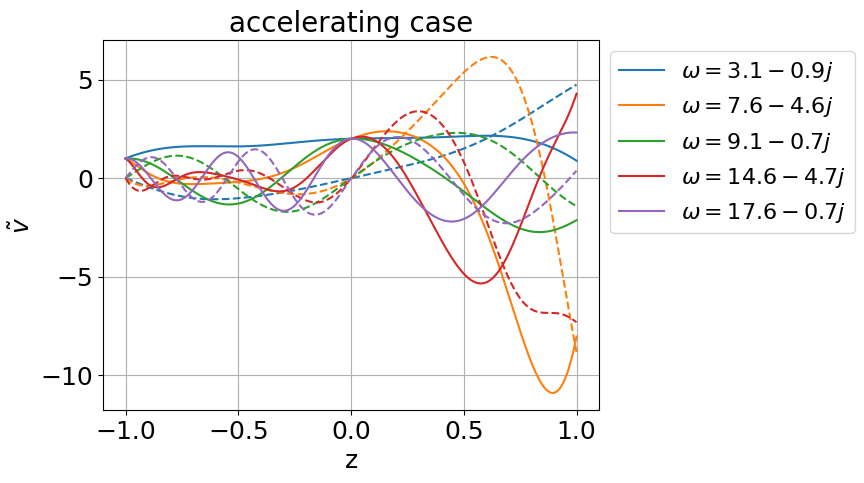
\includegraphics[width=0.95\textwidth]{../../thesis/img/numerical-experiments/accelerating-v-nonzero-bc}
  \caption{By matching the real part of the perturbation to a nonzero real value, we get different eigenvalues and eigenfunctions. What is the physical interpretation of "non-zero" boundary value? How do we interpret these eigenvalues?}
  \label{fig:accelerating-v-nonzero-bc}
\end{figure}

